\documentclass{article}\usepackage{graphicx, color}
%% maxwidth is the original width if it is less than linewidth
%% otherwise use linewidth (to make sure the graphics do not exceed the margin)
\makeatletter
\def\maxwidth{ %
  \ifdim\Gin@nat@width>\linewidth
    \linewidth
  \else
    \Gin@nat@width
  \fi
}
\makeatother

\IfFileExists{upquote.sty}{\usepackage{upquote}}{}
\definecolor{fgcolor}{rgb}{0.2, 0.2, 0.2}
\newcommand{\hlnumber}[1]{\textcolor[rgb]{0,0,0}{#1}}%
\newcommand{\hlfunctioncall}[1]{\textcolor[rgb]{0.501960784313725,0,0.329411764705882}{\textbf{#1}}}%
\newcommand{\hlstring}[1]{\textcolor[rgb]{0.6,0.6,1}{#1}}%
\newcommand{\hlkeyword}[1]{\textcolor[rgb]{0,0,0}{\textbf{#1}}}%
\newcommand{\hlargument}[1]{\textcolor[rgb]{0.690196078431373,0.250980392156863,0.0196078431372549}{#1}}%
\newcommand{\hlcomment}[1]{\textcolor[rgb]{0.180392156862745,0.6,0.341176470588235}{#1}}%
\newcommand{\hlroxygencomment}[1]{\textcolor[rgb]{0.43921568627451,0.47843137254902,0.701960784313725}{#1}}%
\newcommand{\hlformalargs}[1]{\textcolor[rgb]{0.690196078431373,0.250980392156863,0.0196078431372549}{#1}}%
\newcommand{\hleqformalargs}[1]{\textcolor[rgb]{0.690196078431373,0.250980392156863,0.0196078431372549}{#1}}%
\newcommand{\hlassignement}[1]{\textcolor[rgb]{0,0,0}{\textbf{#1}}}%
\newcommand{\hlpackage}[1]{\textcolor[rgb]{0.588235294117647,0.709803921568627,0.145098039215686}{#1}}%
\newcommand{\hlslot}[1]{\textit{#1}}%
\newcommand{\hlsymbol}[1]{\textcolor[rgb]{0,0,0}{#1}}%
\newcommand{\hlprompt}[1]{\textcolor[rgb]{0.2,0.2,0.2}{#1}}%

\usepackage{framed}
\makeatletter
\newenvironment{kframe}{%
 \def\at@end@of@kframe{}%
 \ifinner\ifhmode%
  \def\at@end@of@kframe{\end{minipage}}%
  \begin{minipage}{\columnwidth}%
 \fi\fi%
 \def\FrameCommand##1{\hskip\@totalleftmargin \hskip-\fboxsep
 \colorbox{shadecolor}{##1}\hskip-\fboxsep
     % There is no \\@totalrightmargin, so:
     \hskip-\linewidth \hskip-\@totalleftmargin \hskip\columnwidth}%
 \MakeFramed {\advance\hsize-\width
   \@totalleftmargin\z@ \linewidth\hsize
   \@setminipage}}%
 {\par\unskip\endMakeFramed%
 \at@end@of@kframe}
\makeatother

\definecolor{shadecolor}{rgb}{.97, .97, .97}
\definecolor{messagecolor}{rgb}{0, 0, 0}
\definecolor{warningcolor}{rgb}{1, 0, 1}
\definecolor{errorcolor}{rgb}{1, 0, 0}
\newenvironment{knitrout}{}{} % an empty environment to be redefined in TeX

\usepackage{alltt}
\usepackage{amsmath}
\usepackage{mathtools}
\usepackage{graphicx, color}
\graphicspath{{figs/}}

%----------------------------------
\topmargin      -1.5cm   % read Lamport p.163
\oddsidemargin  -0.04cm  % read Lamport p.163
\evensidemargin -0.04cm  % same as oddsidemargin but for left-hand pages
\textwidth      16.59cm
\textheight     22.94cm
\parskip         7.2pt   % sets spacing between paragraphs
\parindent         3mm   % sets leading space for paragraphs

%-------------------------------------
\title{ Modelling Birds Population }
\author{Ignacio Alvarez}
\date{ Fall 2013 }


\begin{document}
\maketitle 

\section{Introduction} 
According to (REF, Etterson) one of the basic research goals in Ecology consist on understand the distribution and abundance of the animal population. In this work, the particular goal will be to explore alternatives to model the time trends in Western Great Lakes Birds population over 1994 to 2011. 

\vspace{2cm}

\subsection{Data description}

Next table shows total bird count on year 2007 for the most abbundant species, just to compare it with the online annual report. After the table the overall trend for the raw counts over the year are ploted. 

\begin{table}[ht]
\begin{center}
\begin{tabular}{rlrrr}
  \hline
 & abbrev & count.9020 & count.9030 & count.9090 \\ 
  \hline
361 & OVEN & 1003 & 835 & 1168 \\ 
  362 & REVI & 823 & 997 & 771 \\ 
  363 & BTNW & 254 &  &  \\ 
  364 & NAWA & 240 & 348 & 867 \\ 
  365 & BLJA & 222 &  & 230 \\ 
  366 & CSWA & 211 & 330 & 375 \\ 
  367 & RBGR & 208 &  &  \\ 
  368 & WTSP & 180 & 387 & 940 \\ 
  369 & HETH & 175 & 249 & 265 \\ 
  370 & AMRO & 156 &  &  \\ 
  373 & VEER &  & 402 & 264 \\ 
  375 & LEFL &  & 368 &  \\ 
  378 & AMRE &  & 260 &  \\ 
  380 & PIWA &  & 215 &  \\ 
  386 & MAWA &  &  & 282 \\ 
  389 & MOWA &  &  & 257 \\ 
   \hline
\end{tabular}
\end{center}
\end{table}

Forest 9090 (NAMES) is consistently higer than the other two in terms of overal abundance, also it seems to be an increment of the total bird population over time regardless specie.

\begin{figure}[h!]
\centering
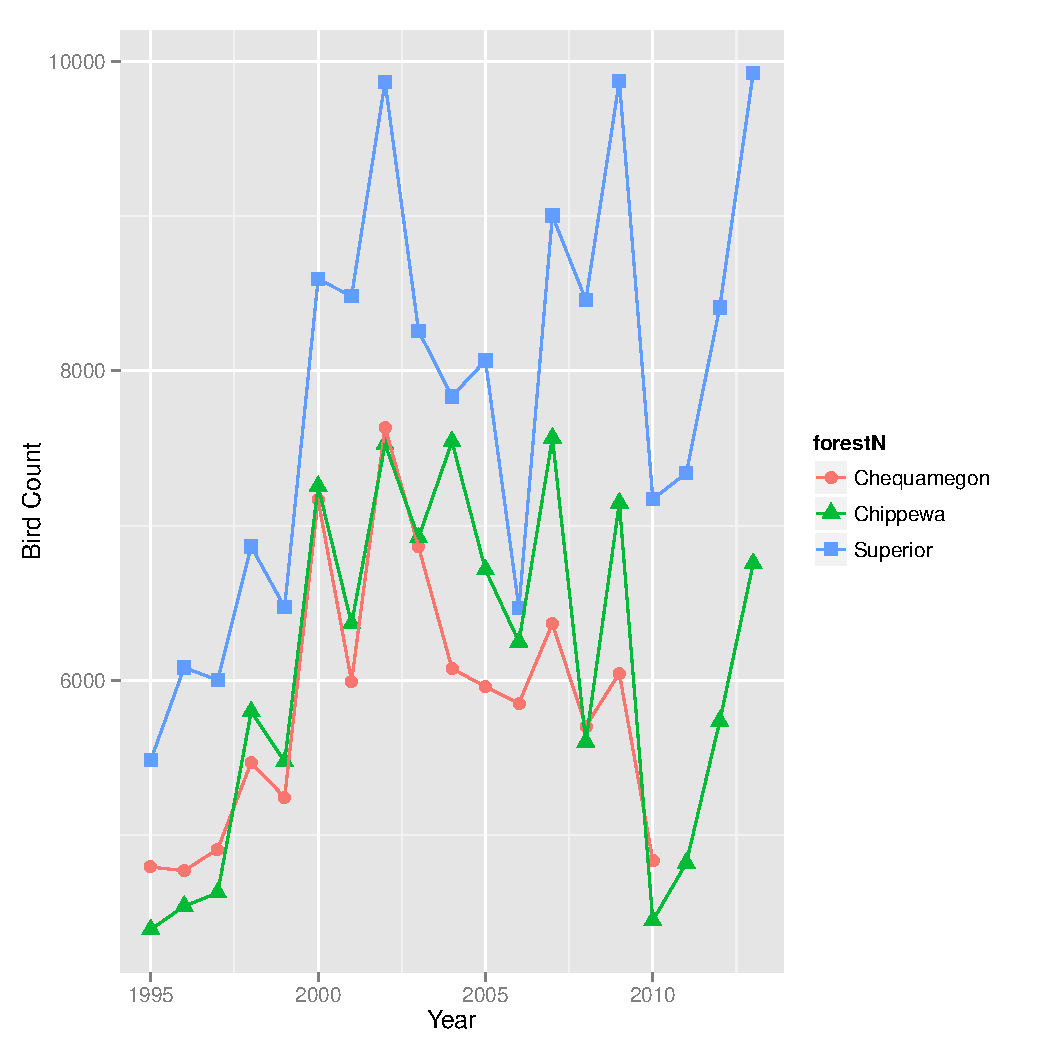
\includegraphics[height=8cm, width=14cm]{rawtrend.pdf}
\caption{Raw trend in the data}
\end{figure}

\subsection{Initial models} 

Perhaps the simplest model we could be a quadratic regression separatedly for each specie and forest. 

\begin{eqnarray}
\nonumber Y_{tfs} &=&  \beta_{0fs} + \beta_{1fs}t + \beta_{2fs}t^2 + \epsilon_{tfs}  \\
\epsilon_{tfs} &\sim& N(0,\sigma^2)
\label{mod1}
\end{eqnarray}

\begin{knitrout}
\definecolor{shadecolor}{rgb}{0.969, 0.969, 0.969}\color{fgcolor}\begin{kframe}
\begin{alltt}
\hlcomment{# ave : average count per year.}
\hlfunctioncall{lm}(ave ~ year + \hlfunctioncall{I}(year^2), data = d)
\end{alltt}
\end{kframe}
\end{knitrout}



where $Y_{tfs}$ represent the average bird count on year $t$ in the forest $f$ for the specie $s$. There are 73 species and 3 forest in the data set so there are 219 models in total. 

Table \ref{tab1} shows the summary statistics for each coefficient and figure \ref{hism1} presents histograms for each one of the model coefficients.

\begin{figure}[h!]
\centering
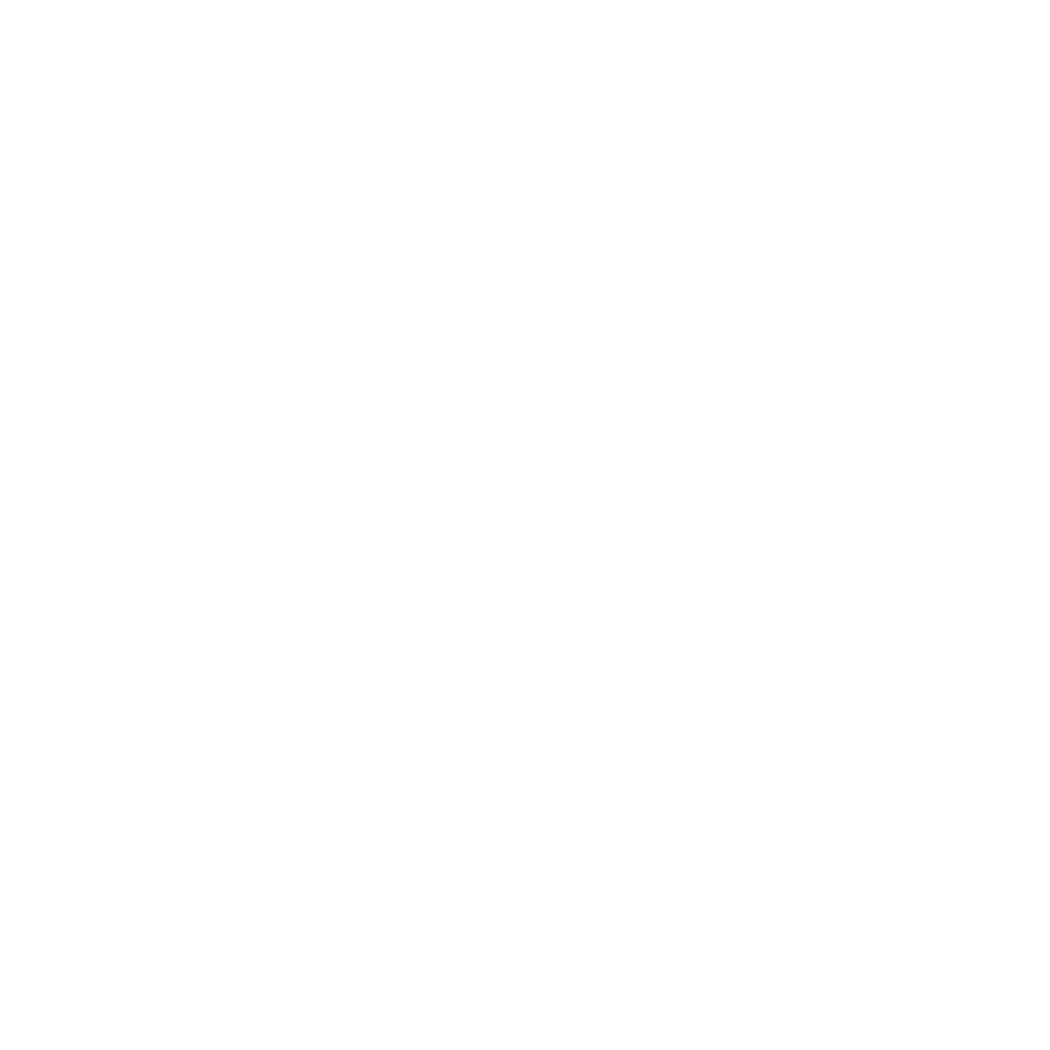
\includegraphics[scale=.6]{hist_m1.pdf}
\caption{Histograms for coefficients of model \ref{mod1}. \label{histm1}}
\end{figure}

\begin{table}[hbpt] 
\caption{Summary stats for coefficients of model \ref{mod1} \label{tab1}}
\begin{center}
\begin{tabular}{rrlrrrrrr} 
  \hline
 & forest & parameter & Min. & 1st Qu. & Median & Mean & 3rd Qu. & Max. \\ 
  \hline
1 & 9020 & b0 & 0.003 & 0.043 & 0.115 & 0.238 & 0.212 & 3.003 \\ 
  2 & 9020 & b1 & -0.012 & 0.001 & 0.003 & 0.010 & 0.011 & 0.140 \\ 
  3 & 9020 & b2 & -0.029 & -0.002 & -0.001 & -0.002 & -0.000 & 0.000 \\ 
  4 & 9020 & sigma & 0.004 & 0.021 & 0.041 & 0.063 & 0.071 & 0.528 \\ \hline
  5 & 9030 & b0 & 0.001 & 0.042 & 0.082 & 0.224 & 0.244 & 2.221 \\ 
  6 & 9030 & b1 & -0.007 & 0.001 & 0.003 & 0.010 & 0.014 & 0.125 \\ 
  7 & 9030 & b2 & -0.015 & -0.001 & -0.000 & -0.001 & -0.000 & 0.001 \\ 
  8 & 9030 & sigma & 0.002 & 0.018 & 0.032 & 0.054 & 0.074 & 0.370 \\ \hline
  9 & 9090 & b0 & 0.000 & 0.015 & 0.072 & 0.217 & 0.223 & 2.407 \\ 
  10 & 9090 & b1 & -0.004 & -0.000 & 0.003 & 0.008 & 0.007 & 0.110 \\ 
  11 & 9090 & b2 & -0.016 & -0.001 & -0.000 & -0.001 & 0.000 & 0.001 \\ 
  12 & 9090 & sigma & 0.001 & 0.011 & 0.028 & 0.054 & 0.070 & 0.349 \\ 
   \hline
\end{tabular}
\end{center}
\end{table}

A second model considered is a regression using data from all 73 species in each forest and including random terms for the species coefficients. 

\begin{eqnarray}
\nonumber log(Y_{tfs}) &=&  \beta_{0fs} + \beta_{1fs}t + \beta_{2fs}t^2 + \epsilon_{tfs}  \\
\nonumber \beta_{0fs} &\sim& N(\beta_{0f}, \sigma_{0f}^2 ) \\ 
\nonumber \beta_{1fs} &\sim& N(\beta_{1f}, \sigma_{1f}^2 ) \\ 
\nonumber \beta_{2fs} &\sim& N(\beta_{2f}, \sigma_{2f}^2 ) \\ 
\epsilon_{tfs} &\sim& N(0,\sigma^2)
\label{mod2}
\end{eqnarray}

\begin{knitrout}
\definecolor{shadecolor}{rgb}{0.969, 0.969, 0.969}\color{fgcolor}\begin{kframe}
\begin{alltt}
\hlcomment{# ave : average count per year.}
\hlfunctioncall{library}(lme4)
\hlfunctioncall{lmer}(ave ~ year + \hlfunctioncall{I}(year^2) + (year + \hlfunctioncall{I}(year^2) | abbrev), data = d)
\end{alltt}
\end{kframe}
\end{knitrout}



\begin{figure}
\centering
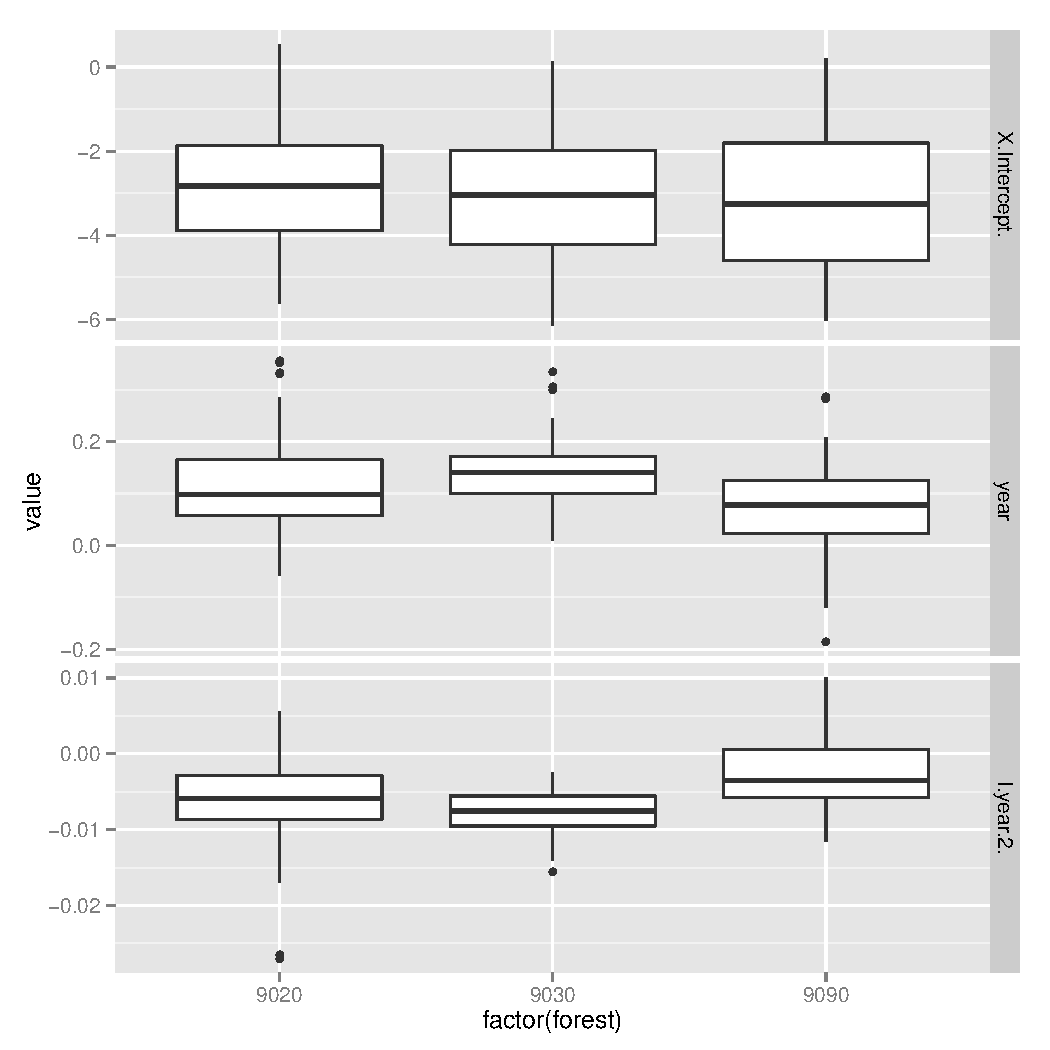
\includegraphics[scale=.45]{box_m2.pdf}
\caption{Boxplots for random effects in model \ref{mod2}. \label{boxm2}}
\end{figure}

\begin{table}[ht]
\caption{Estimated mean and variance in model \ref{2}}
\begin{center}
\begin{tabular}{rrlrr}
  \hline
 & forest & parameter & mean & variance \\ 
  \hline
1 & 9020 & b0 & -2.900 & 1.462 \\ 
  2 & 9020 & b1 & 0.119 & 0.126 \\ 
  3 & 9020 & b2 & -0.007 & 0.008 \\ 
  4 & 9020 & residual & 0.000 & 0.487 \\ \hline
  5 & 9030 & b0 & -3.131 & 1.602 \\ 
  6 & 9030 & b1 & 0.143 & 0.090 \\ 
  7 & 9030 & b2 & -0.008 & 0.004 \\ 
  8 & 9030 & residual & 0.000 & 0.496 \\ \hline
  9 & 9090 & b0 & -3.236 & 1.704 \\ 
  10 & 9090 & b1 & 0.067 & 0.121 \\ 
  11 & 9090 & b2 & -0.003 & 0.006 \\ 
  12 & 9090 & residual & 0.000 & 0.518 \\ 
   \hline
\end{tabular}
\end{center}
\end{table}


\newpage

\section{Statistical Model} 

\begin{eqnarray}
\nonumber log(Y_{tfs}) &=&  \beta_{0fs} + \beta_{1fs}t + \beta_{2fs}t^2 + \epsilon_{tfs}  \\
\nonumber \beta_{fs} &=& \left(\begin{array}{c}
    \beta_{0fs}   \\ 
    \beta_{1fs}  \\ 
    \beta_{2fs}  
\end{array}\right) \sim N(0, \Sigma_{fs}) \\
\nonumber \Sigma_{fs}  &\sim& \mbox{inv-gamma, scaled inv-gamma, ...} \\ 
\nonumber \epsilon_{tfs}  &\sim& N(0,\sigma_{\epsilon}^2) \\
\nonumber \sigma_{\epsilon}^2  &\sim& inv-gama(\alpha,\gamma) \\
\label{mod3}
\end{eqnarray}






%%%%%%%%%%%%%%%%%%%%%%%%%%%%%%%%%%%%%%%%%%%%%%%%%%%%%%%%%%%%%%%%%%%%%%%%
\end{document}
